\newacronym{HTTP}{$HTTP$}{Hypertext Transfer Protocol}
\glsadd{HTTP}
\newacronym{TCP}{$TCP$}{transmission Control Protocol}
\glsadd{TCP}
\newacronym{API}{$API$}{Application Programming Interface}
\glsadd{API}
\newacronym{PCD}{$PCD$}{Proximity coupling device}
\glsadd{PCD}
\newacronym{PICC}{$PICC$}{Proximity Integrated circuit card}
\glsadd{PICC}
\newacronym{IaaS}{$IaaS$}{Infrastructure as a service}
\glsadd{IaaS}
\newacronym{PaaS}{$PaaS$}{Platform as a service}
\glsadd{PaaS}
\newacronym{SaaS}{$SaaS$}{Software as a service}
\glsadd{SaaS}
\newacronym{SQL}{$SQL$}{Structured Query Language}
\glsadd{SQL}
\newacronym{UART}{$UART$}{Universal Asynchronous Receiver-Transmitter}
\glsadd{UART}
\newacronym{URL}{$URL$}{Uniform Resource Locator}
\newacronym{GPIO}{$GPIO$}{General Purpose Input Output}
\glsadd{GPIO}
\newacronym{12C}{$12C$}{Inter-Integrated Circuit}
\glsadd{12C}
\newacronym{SPI}{$SPI$}{Serial Peripheral Interface}
\glsadd{SPI}

\chapter{Background}
\section*{Project Specification}
The monitoring system is split into three different parts which includes the website, raspberry pi and the cloud(Azure). These are also split in their respective parts with the website containing the web server(node) and the site(React), the Cloud; Azure sql server and Azure sql database
 
\section{Website}
A website is often confused with a web page or a web server. According to \cite{Whatisth32:online}, A website is a collection of web pages which are grouped together in various ways. A web server is a computer that hosts websites and their supporting files, which are available on that computer. From a web developer point of view the webpages are known as the clients while the web servers are known as the servers. The clients are copies downloaded from the server
 
 
\subsection{Communication between clients and servers}
\begin{itemize}
 \item \textbf{Internet Connection}: This enables the transmission of data between clients and server
 \item \textbf{TCP/IP}: These are communication protocols that define how data should be transmitted on the internet. IP handles the delivery of packets of information from source to destination while TCP handles the management of these packets by joining them together in their right order and also asks for missing packets to be resent, this retransmission causes latency.
 \item \textbf{HTTP}: This is an application layer protocol that determines how clients and server communicate.
\end{itemize}
 

A website talks to the web server using an API, which is a connection between computer programs. It could be referred also as the specification or as the implementation, the specification has to do with a document that demonstrates how to use or create a connection. Examples of API specifications used in this project are; tedious for the database connection to azure, express as a middleware. An API rule says that you should get a resource when you link; to a unique URL. The resource is a chunk of data, and is gottend in the form of a response, the URL is in the form a request. A request consists of mainly four things, the endpoint, the method, the header, the data;
\begin{itemize}
  \item The endpoint: it is one end of a communication where a function or a resource can be rendered when invoked. it is the url requested for, each endpoint returns a unique resource
  \item The method: the type of request to send the server, There are variant types used, but the well-known types are:
  \begin{center}
    \begin{tabular}{|c|   c   |}
      \hline
      \textbf{HTTP method} & function\\
      \hline
      GET & request to retrieve resources from the server\\
      \hline
      POST & request to create a new resource on a server\\
      & this could be stored on a database or used as a\\
      & variable for a function\\
      \hline
      PUT & request used to update a resource on a server\\
      \hline
      DELETE & request used to delete a resource referenced\\
      \hline
    \end{tabular}
  \end{center}
  \item header: this contains information about the request and is useful to both the client and the server. It can serve as a means of authentication and to understand the contents of the body. Headers are categorized according to their contexts:
  \begin{itemize}
    \item \textbf{request header} provides information about request to the server
    \item \textbf{response header} provides information about the response gotten from the server
  \end{itemize}
  \item The data/body: contains information required by the server, a GET request doesn't carry a body.
\end{itemize}


\textbf{HTTP status codes}: these represent the outcome of a request, they are responses. Responses are mainly grouped in five according to \cite{HTTPresp7:online}:  informational response is between \textit{100 - 199}, a successful response is between \textit{200 - 299}, a Redirection message \textit{300 - 399}, a client error response \textit{400 - 499} and server error response \textit{500 - 599}.
\begin{center}
  \begin{tabular}{|c|  c   |}
    \hline
    \textbf{HTTP code} & meaning\\
    \hline
    200 & Ok, the request succeeded\\
    \hline
    400 & Bad request, the server cannot process\\
    &the request due to a client error\\
    \hline
    404 & Not Found, the server cannot\\
    &find the requested resource\\
    \hline
    405 & Method Not Allowed, the method\\
    &is recognised but is not allowed by the server\\
    \hline
    500 & Internal Server Error, the server\\
     &does not know how to handle a request\\
    \hline
  \end{tabular}
\end{center}

 
\section{Raspberry-pi}
A portable computer with 40 GPIO pins, a dedicated processor, memory, graphics driver and an operating system, raspbian OS which is similar to most linux distro's. The raspberry pi 4 runs on a range \cite{Arduinov52:online}
GPIO is an uncommitted digital pin on an electronic circuit board which may be used as input or output or both, and can be configured by the user at runtime[6]. This GPIO allows to interface with different modules. A module here is a small unit that can be integrated into a larger system but also maintained separately with no effect on the system. It is of a "plug-in" functionality.
To connect to azure from the raspberry pi, "pyodbc" driver is used. The driver files are installed on the raspberry-pi
LED  

\subsection{RFID - RC522}
\subsubsection{Interfacing with the Rasberry pi}
The RFID card interfaces with the raspberry-pi with SPI communication but is also compatible with 1\textsuperscript{2}C and UART communication, it is a synchronous serial communication that encourages communication over a short distance, it is mainly used in embedded systems. Serial communication has to do with sending one bit at a time sequentially and synchronous means that this communication is synchronized by a clock signal which is used orchestrate the actions of the digital circuit i.e to determine when it is time to read the next bit/value. SPI devices communicate in a full duplex mode with a master-slave principle normally with a single master. full duplex means that data is transmitted back and forth simultaneously in this communication channel.

\textit{Note: The master is the raspberry pi.}
\vspace{1cm}
\begin{figure}[ht]
  \centering
  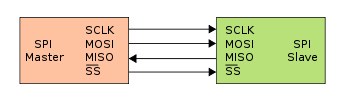
\includegraphics{Background/images/350px-SPI_single_slave.svg.png.png}
  \caption{SPI master slave architecture}
\end{figure}
\vspace{1cm}

SPI has four main logic signals: 
\begin{itemize}
  \item SCLK: Serial clock, which accepts pulses obtained from the master
  \item MOSI: Master Out Slave In, this is data transmitted from the master to slave
  \item MISO: Master In Slave Out, this is data transmitted from the slave to master
  \item CS/SS: Chip/Slave Select, an output from the master to notify data is being transmitted.
\end{itemize}

The RC522 module has 8 pins that interfaces with the raspberry pi;
\begin{itemize}
  \item SDA: 1\textsuperscript{2}C-bus serial data line input/output, it acts as as signal input when used for SPI communication
  \item SCK: SPI serial clock input which has the same operation as SCLK
  \item RST: an input for Reset and power-down of the module. It can turn off all the input pins and internal current sinks. 
  \item GND: for ground connection to the GPIO pin of the master
  \item IRQ: an interruption pin, that could notify the master when an RFID tag comes into the range of scan.
  \item 3.3v/VCC: which powers the RC522 module
  \item MOSI: has the same operation as MISO in SPI communication, receives data from master
  \item MISO: has the same operation as MOSI in SPI communication, sends data to master(raspberry pi)
\end{itemize}

\subsubsection{Operations of RFID module}
RFID tags are classified by their frequencies, the four primary frequency ranges are:
\begin{itemize}
  \item Low frequency (LF): they are frequencies from 30 to 300KHz
  \item High frequency (HF): frequencies are from 3 to 30MHz, has a higher memory size and a longer range of transmission
  \item Ultra high frequency (UHF): frequencies are from 300MHz to 3GHz
  \item Microwave frequency (microwave): they function at 2.45GHz 
\end{itemize}
The system consists of two main components, a transponder/tag and a transceiver/reader or a PCD and a PICC as defined in ISO 14443. The transceiver creates a 13.56MHz electromagnetic field that communicates with the tag. 
This project uses a High Frequency passive card with Type A communication defined in ISO-14443, passive meaning, the tags only function when they acquire signals from a reader and relay an information-carrying signal back to the reader. 


\subsection{Fingerprint - JM-101}
The JM-101 comes with a flash memory to store the fingerprints, it has a storage capacity of over 300 templates. 
\subsubsection{Interfacing with Raspberry pi}
The Fingerprint interfaces with the Raspberry pi with UART communication, it is a devices that supports asynchronous serial communication, which is a form of serial communication that doesn't require a clock signal and is not constantly synchronized. Raspberry pi supports asynchronous communication but with a lot of fingerprints having distinct voltages, I used a USB to UART Converter which supports both 3.3v and 5v although the JM-101 is 3.3v. The TX pin goes to RX pin and vice versa in the connection between the converter and fingerprint module. The USB to UART Converter goes into the USB port of the raspberry pi while its pins are connected to the pins of the fingerprint module.
The pins used in interfacing with the UART converter are:
\begin{itemize}
  \item GND: ground connection
  \item RXD: the receiver of data
  \item TXD: transmits data
  \item 3V3: powers the fingerprint module
\end{itemize}

\subsubsection{Operations of fingerprint module}
Fingerprint processing can either be for enrollment or matching, The user enters his finger two times when enrolling, the two templates are used to generate a template after being processing their results. 
A matching algorithm is used to compare fingerprint templates stored in the flash memory with the one read by the fingerprint module. There are two types of matching; 1:1 and 1:N. In 1:1 the module compares the read fingerprint with a pre-existing template that is specified in the code while 1:N checks the read fingerprint with all templates previously stored in the flash memory.


\subsection{Flask}
This creates a local server written in python. It has a feature that binds a python function to a URL endpoint. Another feature of flask is its ability to handle multiple request with one function. It is like a switch or if-else condition: if it is a POST it executes a function but if it is a GET it executes another function.

\subsection{Virtual tunnel}
pitunnel is used to connect the Flask Server with the NodeJS server this is used for development purposes. The Flask server alone runs locally and has no access to the Internet, pitunnel is a service that allows access to any network service on the raspberry pi from anywhere in the world. In my project the service used is http all, that is needed is to configure pitunnel to track the localhost server running and you can use the pitunnel endpoint to receive data on the raspberry pi. Pitunnel does this by mirroring the flask server: the root directory of the flask server becomes the root directory of the Pitunnel same as other endpoints when calling an endpoint of the flask server.  

\section{Cloud - Azure}
Cloud computing has to do with the provision of computing system resources like data storage, servers, software over the internet\cite{Cloudcom53:online}. The benefits of these include reliability: the cloud provider is in charge of handling data and handles data back-up by mirroing these data at different locations, Scalability: the ability for you to "scale up" when there is an increase in demand for computing power, also provides the appropiate amount of resource for a task.
There are different types of clouds and they have unique functions;
\begin{itemize}
  \item Public cloud: these are delivered over the internet by third-party providers like Microsoft Azure, Amazon Web Services etc.
  \item Private cloud: its resources are solely designed for a single organization, these can be handled by a third-party or hosted by that organization and located on their own personalized data centre.
  \item Hybrid cloud: a combination of a private and public cloud and aims to give the user more flexibility. An organisation could host a private cloud with sensitive data and connect with a public cloud to host its application
\end{itemize}

These clouds provide their services according to models, there are mainly three according to of these models\cite{National40:online};
\begin{itemize}
  \item \gls{IaaS}: this provides the user with resources like virtual machines, storage, operating systems
  \item \gls{PaaS}: provides the user with an environment to develop software with out management of the underlying resources required like servers, operating systems
  \item \gls{SaaS}: the cloud provider supply users with software over the Internet, this is mostly done by connection to a web browser, here the consumer does not management the underlying resources 
\end{itemize}

\begin{figure}[ht]
  \centering
  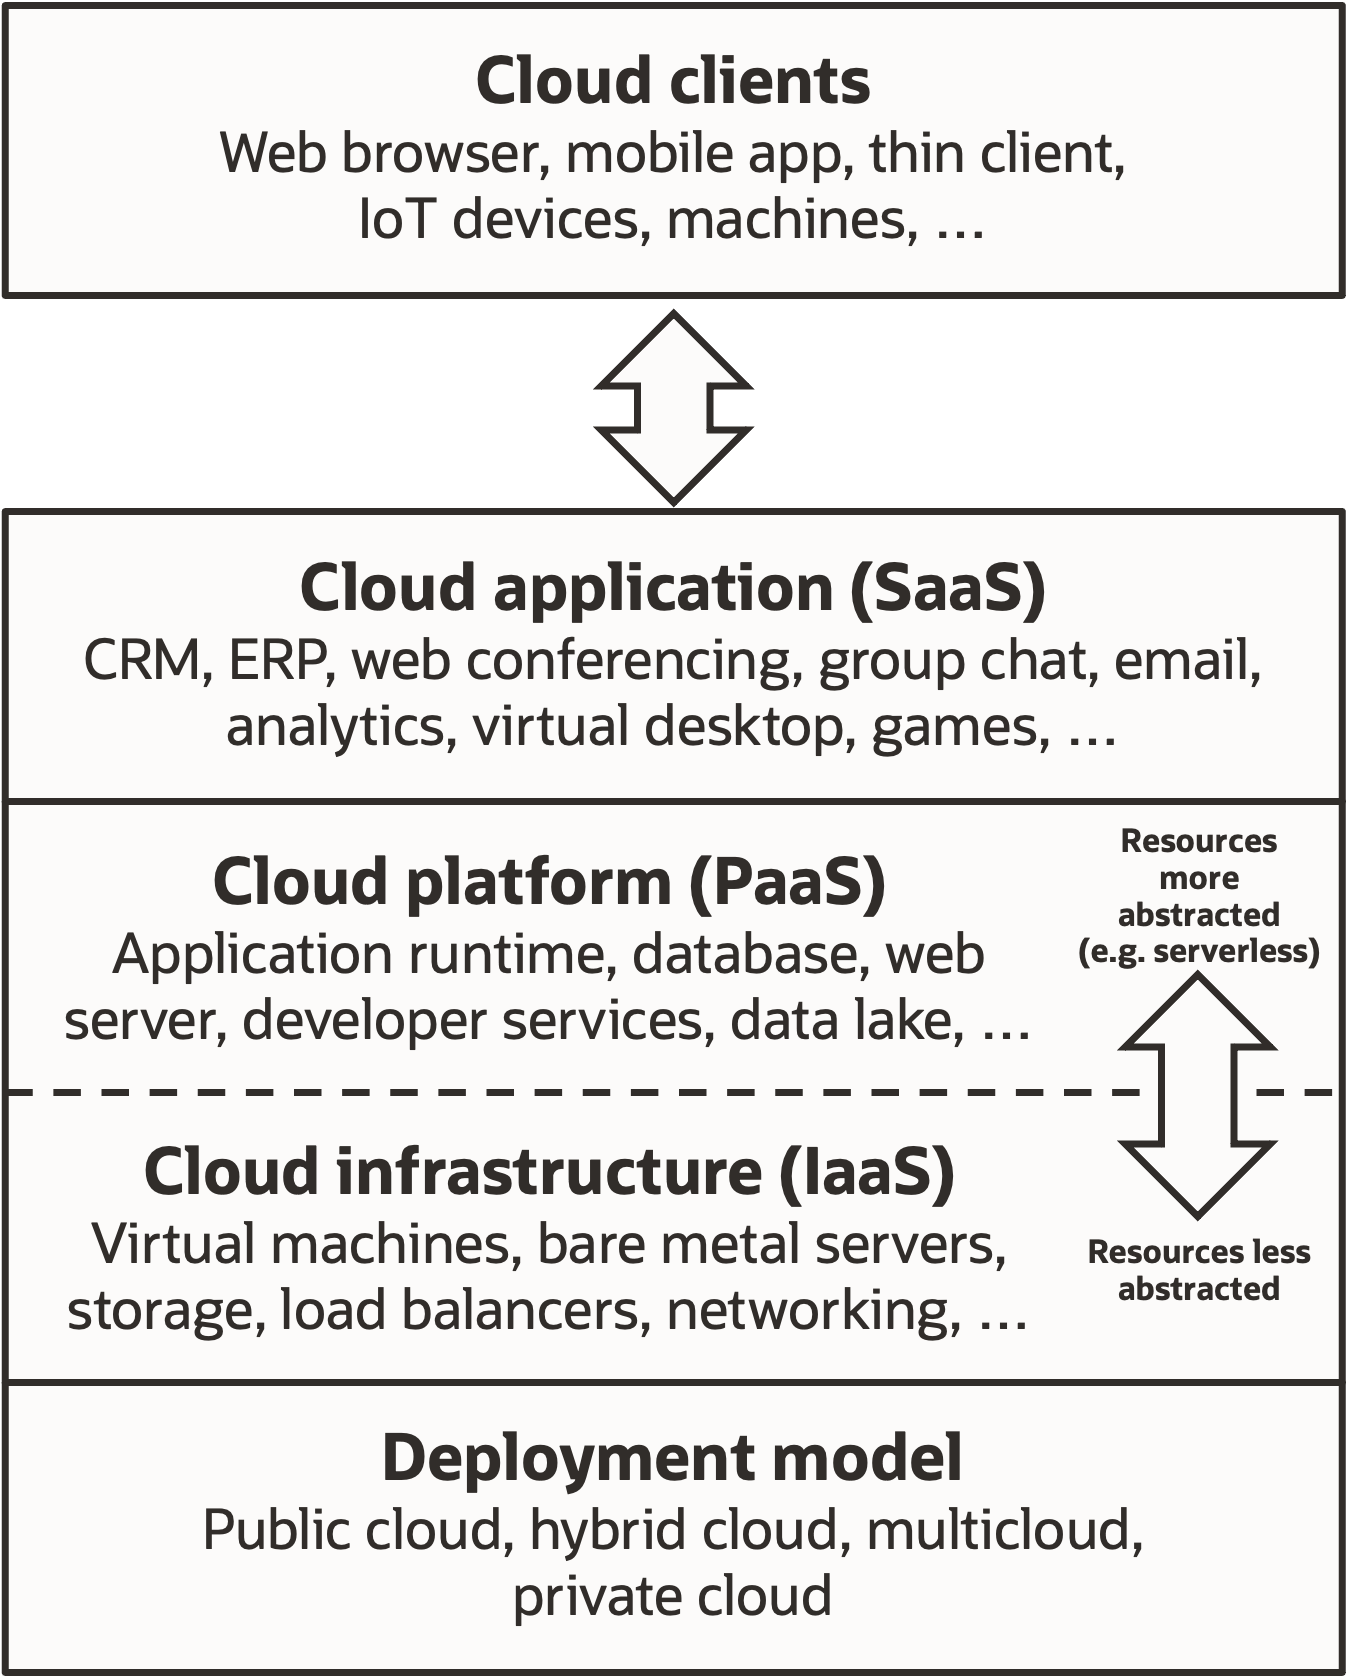
\includegraphics[scale=0.8]{Background/images/Cloud_computing_service_models_(1).png}
  \caption{Cloud computing service models arranged as layers in a stack \cite{Cloudcom53:online}}
\end{figure}
This project uses public cloud type provided by Microsoft Azure and IaaS for my storage and PaaS for my server. AzureSQL server hosts the SQL database and handles connection to other devices, programs or services. 
My options where NoSQL("Not Only SQL") or SQL also known as Sequel.
SQL is a programming language used to manage data in a relational database, I specifically used T-SQL for querying data in Microsoft SQL Server. 

\subsection{Terms Used}
A lot of these terms will be used to talk about managing the database;

\begin{itemize}
  \item Table: they contain all data in database, they do this in the form of a row and column format, where each row is a unique record and each column a unique attribute
  \item Rows: represents a collection of attributes that make up a data record 
  \item Columns: They represent different attributes of a table, a single column has a similar data type for all rows.
  \item Primary key: it is a column or a group of columns that acts as an identifier of each rows of a table.
  \item Foreign key: it can be a column or a group of columns that allows a link between two related tables by referring to the Primary Key of another table
\end{itemize}

\subsection{Communication between the Database and other devices}
The azure web portal provides a list of connection strings to interact with the sql database, for my project I used the ODBC driver with SQL authentication connection string:
\begin{verbatim}
  Driver={ODBC Driver 13 for SQL Server};
  Server=tcp:csproj.database.windows.net,1433;
  Database=vantracker;
  Uid=g3ar;
  Pwd={your_password_here};
  Encrypt=yes;
  TrustServerCertificate=no;
  Connection Timeout=30;
\end{verbatim}




